
\documentclass{sig-alternate-2013}

\usepackage{url}
\usepackage[english,french]{babel}
\usepackage[utf8]{inputenc}
%%\usepackage[T1]{fontenc}
\usepackage{algorithm}
\usepackage{paralist}
\usepackage{algorithmicx}
\usepackage{algpseudocode}

%%\usepackage{amsfonts}
\usepackage{fancyhdr}
\usepackage{graphicx}
\usepackage{hyperref}                                  
\usepackage{multirow}
%%\usepackage{multicol}
%\usepackage{todonotes}
\usepackage{epstopdf}
\usepackage{epsfig}

%%\usepackage{amsthm}

%% Bibtex
\usepackage[numbers]{natbib}

\usepackage{tikz}
\usetikzlibrary{plotmarks,shapes}
%%\usepackage{geometry}

%\usepackage{subfigure}
\usepackage{subcaption}
%\usepackage[small]{caption}

%%\geometry{vmargin=1.5cm, hmargin=1.0cm}

\newcommand{\TOFIX}[1]{\textcolor{orange}{#1}}
\newcommand{\TODO}[1]{\textcolor{red}{#1}}
\newcommand{\ELEM}[1]{\textcolor{blue}{#1}}
\newcommand{\NAME}[0]{\textit{h}-LSEQ}

%paralist
\renewcommand*\descriptionlabel[1]{%
\scshape #1}
\renewcommand\paradescriptionlabel[1]{%
\scshape #1}


\hypersetup{
  colorlinks,
  citecolor=black,
  filecolor=black,
  linkcolor=black,
  urlcolor=black
}

\title{Concurrency Effects Over Variable-size Identifiers in Distributed
  Collaborative Editing}


\numberofauthors{1}
\author{
     \alignauthor Brice Nedelec, Pascal Molli, Achour Mostefaoui, Emmanuel Desmontils\\
     \affaddr{LINA, 2 rue de la Houssini\`ere}\\
     \affaddr{BP92208, 44322 Nantes Cedex 03}\\
     \email{first.last@univ-nantes.fr}
}

\date{}

%%\input{input/data/indexdata.tex}

\permission{This work is licensed under the Creative Commons
  Attribution-ShareAlike~3.0 Unported License (CC BY-SA 3.0). To view a copy of
  the license, visit http://creativecommons.org/licenses/by-sa/3.0/. \\}
\conferenceinfo{DChanges 2013,}{September 10th, 2013, Florence, Italy.}
\copyrightetc{ceur-ws.org \the\acmcopyr} \crdata{Volume 1008,
  http://ceur-ws.org/Vol-1008/paper5.pdf}


\begin{document}
\newtheorem{Def}{Definition}

\selectlanguage{english}

  \maketitle

  
\begin{abstract}

  Distributed collaborative editors such as Google Docs or Etherpad allow to
  distribute the work across time, space and organizations. In this paper, we
  focus on distributed collaborative editors based on the Conflict-free
  Replicated Data Type approach (CRDT). CRDTs encompass a set of well-known
  data types (sets, graphs, sequences, etc.). CRDTs for sequences model a
  document as a set of elements (character, line, paragraph, etc.) with unique
  identifiers, providing two commutative update operations: insert and
  delete. The identifiers of elements can be either of fixed-size or
  variable-size. Recently, a strategy for assigning variable-size identifiers
  called LSEQ has been proposed for CRDTs for sequences. LSEQ lowers the space
  complexity of variable-size identifiers CRDTs from linear to
  sub-linear. While experiments show that it works locally, it fails to provide
  this bound with multiple users and latency. In this paper, we propose
  \NAME{}, an improvement of LSEQ that preserves its space complexity among all
  collaborators, regardless of the latency. Ultimately, this improvement allows
  to safely build distributed collaborative editors based on CRDTs. We validate
  our approach with simulations involving latency and multiple users.


\end{abstract}

%%% Local Variables: 
%%% mode: latex
%%% TeX-master: "../dchanges"
%%% End: 

  \category{I.7.1}{Document and Text
  Processing}{Document and Text Editing}[Document management]
\category{C.2.4}{Computer-Communication Networks}{Distributed
  Systems}[Distributed applications]
\category{D.2.8}{Software Engineering}{Metrics}[Complexity measures]


\keywords{Distributed Documents; Document Authoring Tools and Systems;
  Distributed Collaborative Editing; Real-time Editing; Conflict-free
  Replicated Data Types}

  \newpage
  
\section{Introduction}

Distributed collaborative editors allow to distribute the work across space,
time and organizations. Some trending editors such as Google
Docs~\cite{nichols1995high} use the Operational Transform (OT)
approach~\cite{sun1998operational,sun1998achieving}. However, an alternative
based on Conflict-free Replicated Data Types
(CRDTs)~\cite{shapiro2011comprehensive,shapiro2011conflict} exists.  Compared
to OT, CRDTs are more decentralized and scale better.

The CRDTs belong to the optimistic
replication~\cite{saito2002replication,saito2005optimistic}
approach. Therefore, replicas involved in the collaboration are guaranteed
eventual convergence to an identical state. To provide convergence in a
replicated sequence, CRDTs use unique identifiers to link elements. When the
sequence is a document, the elements can be characters, lines, paragraphs, etc.


We distinguish two types of sequence CRDTs:
\begin{inparaenum}[(i)]
\item The tombstone
  CRDTs~\cite{ahmed2011evaluating,grishchenko2010deep,oster2006data,preguica2009commutative,roh2011replicated,weiss2007wooki,wu2010partial,Yu2012stringwise}
  use fixed-size identifiers. However, the delete operations only mark and hide
  elements to the users. Consequently, these deleted elements permanently
  affect performances.
\item The variable-size identifiers
  CRDTs~\cite{preguica2009commutative,weiss2009logoot} directly encode the
  order relation in the identifiers. However, their identifiers can grow
  linearly depending on the editing behaviour. Consequently, they remain unsafe
  in the distributed collaborative editing context.
\end{inparaenum}

To overcome their respective limitations, these approaches need an additional
protocol~\cite{letia2009crdts,roh2011replicated} related to garbage collection
mechanisms. Nevertheless, these protocols require global knowledge over
participants. In the general case, such knowledge remains prohibitively
expensive in the context of distributed networks subject to churn.

Recently, LSEQ~\cite{nedelec2013lseq} allowed variable-size identifiers CRDTs
to get rid of this costly additional protocol by lowering their upper bound on
space complexity from linear to sub-linear. Yet, LSEQ does not guarantee a safe
allocation. Indeed, it uses multiple antagonist strategies which, without any
coordination between collaborators, leads to an quadratic growth of
identifiers.

The contributions of this paper are:
\begin{inparaenum}[(i)]
\item experiments that highlight the negative effect of multiple users edition
  on the size of LSEQ identifiers
\item experiments that highlight that an increasing latency does not have a
  negative impact on the size of LSEQ identifiers.
\item an improvement of LSEQ called \NAME{} that extends the single user
  sub-linear upper bound on space complexity to any number of users, regardless
  of the latency, and without any additional cost.
\end{inparaenum} 

Ultimately, \NAME{} allows distributed collaborative editors to safely use
variable-size identifiers CRDTs.

The rest of the paper is organized as follow: Section~\ref{sec:background}
details variable-size identifiers CRDTs for sequences, the allocation strategy
LSEQ, and highlights the motivation of this paper.  Section~\ref{sec:proposal}
presents \NAME{} a combination of LSEQ and a hash-based choice strategy to
overcome the LSEQ limitations.  Section~\ref{sec:experiments} shows the results
of experiments over LSEQ and \NAME{} considering latency and multiple
users. Finally, Section~\ref{sec:relatedwork} reviews the related works.


%%% Local Variables: 
%%% mode: latex
%%% TeX-master: "../dchanges"
%%% End: 

  
\section{background}
\label{sec:background}

Conflict-free Replicated Data Types belong to the optimistic
replication approach~\cite{saito2002replication,saito2005optimistic}. In the
context of distributed collaborative editing, the replicated data is a
document, where:
\begin{inparaenum}[(1)]
\item each insert/delete operation is prepared locally and broadcast,
\item each remote replica receives and integrates the change,
\item all involved replicas eventually converge to an identical state.
\end{inparaenum}

To provide the convergence property, CRDTs for sequences model a document as a
set of couples $\langle elt, id\rangle$ where $id \in (\mathcal{I}, <_{id})$,
$<_{id}$ being a strict and dense total order, and $elt$ any element
(e.g. character, line, etc.). Two commutative operations allow to update the
document:
\begin{itemize}
\item $insert(p \in \mathcal{I}, elt, q \in \mathcal{I})$ that generates an
  identifier $id_{elt}$ with $p<id_{elt}<q$ and adds $\langle elt, id_{elt}
  \rangle$ to the document.
\item $delete(id_{elt})$ that removes $\langle elt, id_{elt}\rangle$ from the
  document.
\end{itemize} 

The variable-size identifiers
CRDTs~\cite{preguica2009commutative,weiss2009logoot} define identifiers as a
series of numbers that can designate paths in a tree. An allocation strategy is
in charge of choosing these sequences of numbers. It aims to keep these
identifiers as small as possible for the sake of performances.

\begin{figure}[h]
\begin{center}
\begin{tikzpicture}[scale=1.0]
\tiny

  
  \draw (0,0) -- node[anchor=south east]{0}  (-85pt, -50pt);
  \draw (0,0) -- node[anchor=south west]{99} ( 85pt, -50pt);

  \draw (0,0) -- node[anchor=east]{20} (-60pt, -50pt);
  \draw (0,0) -- node[anchor=east]{21} (-20pt, -50pt);
  \draw (0,0) -- node[anchor=east]{50} ( 30pt, -50pt);

  \draw[fill=white] (0,0) circle (1pt);

  \draw[<->,color=red] (32pt,-50pt) -- node[anchor=north]{(1)} (83pt, -50pt);


\small
  \draw[fill=white] (-85pt, -50pt) node[anchor=north]{Begin} circle (1pt);
  \draw[fill=white] ( 85pt, -50pt) node[anchor=north]{End} circle (1pt);

\tiny
  \draw (-60pt,-50pt) -- node[anchor=east]{10} (-50pt, -100pt);
  \draw (-60pt,-50pt) -- node[anchor=west]{11} (-40pt, -100pt);

  \draw[<->,color=red] (-48pt,-100pt) -- node[anchor=north]{(2)} (-42pt,
  -100pt);

\small
  \draw[fill=black] (-60pt, -50pt) circle (1pt);
  \draw[fill=black] (-20pt, -50pt) circle (1pt);
  \draw[fill=black] ( 30pt, -50pt) circle (1pt);

  \filldraw[black](-50pt, -100pt) circle (1pt);
%  \filldraw[black] (-30.8pt, -100pt) node[anchor=north]{23} circle (1pt);
  \filldraw[black](-40pt, -100pt) circle (1pt);
%  \filldraw[black] (-12.0pt, -100pt) node[anchor=north]{70} circle (1pt);
%  \filldraw[black](- 3.2pt, -100pt) circle (1pt);


\end{tikzpicture}

\end{center}
\caption{Underlying 100-ary tree model of variable-size identifiers CRDTs. It
  contains 5 identifiers. 3 identifiers at depth-1: [20], [21], [50] and 2
  identifiers at depth-2: [20.10], [20.11]. For the simplicity purpose, the
  element linked to identifiers are not displayed.}
\label{fig:treeexample}
\end{figure}

Figure~\ref{fig:treeexample} illustrates the underlying model of variable-size
CRDTs.  If an insertion operation is performed at (1), the allocation strategy
chooses an identifier [X] with $50<X<99$. When the insert operation is
performed at (2), there is no room for another identifier, therefore, the new
identifier will be a sequence of three numbers: [20.10.X], where $0<X<100$.

These identifiers can grow linearly depending on the position of insert
operations.

Recently, LSEQ~\cite{nedelec2013lseq} lowered the space complexity of these
CRDTs from linear to sub-linear without favouring any editing behaviour. This
improvement aims to get rid of the previously mandatory garbage collecting
protocol. Three components compose LSEQ:
\begin{itemize}
\item{base doubling:} regarding the underlying tree model, each node can have
  twice more children than its parent. It follows the properties of exponential
  trees~\cite{andersson2007dynamic}.
\item{two antagonist allocation strategies:} \emph{boundary+} and
  \emph{boundary--} that are designed for end-edition and front-edition
  respectively.
\item{random strategy choice:} it randomly assigns an allocation strategy to
  each depth of the tree. It follows the intuition: \emph{since we have no
    prior knowledge of the editing behaviour, the strategy choice should not
    favor any editing behaviour. Consequently, the frequencies of appearance of
    each allocation strategy have to be equal.}
\end{itemize}

Despite the fact that numerous experimentation have been performed on LSEQ
including real documents extracted from Wikipedia, they did not include any
concurrency. Indeed, Wikipedia's revisions already present a serialization of
the document, without explicit concurrency. Although, the
paper~\cite{ahmed2011evaluating} highlighted the importance of such documents.

\begin{table}[h]
  \begin{center}
    \begin{tabular}{|l|r|r|r|r|r|}
      \cline{2-6}
      \multicolumn{1}{c|}{} & \multicolumn{5}{c|}{\textbf{\#insert operations}}
      \\
      %%\cline{2-6}
      \multicolumn{1}{c|}{} & \textbf{10} & \textbf{100} & \textbf{200}
      & \textbf{500} & \textbf{1000} \\
      \hline
      1 user (bit/id) & 6.5 & 26.8 & 32.7 & 56.0 & 64.2 \\
      \hline
      10 users (bit/id) & 9.5 & 125.8 & 377.0 & 1962.1 & 5468.0 \\
      \hline
    \end{tabular}
    \caption{Experimentation on the average bit-length of LSEQ identifiers
      with 1 user and 10 collaborators generating a document of 10, 100, 200,
      500, and 1000 lines.}
    \label{tab:motivating}
  \end{center}
\end{table} 

Table~\ref{tab:motivating} shows the average bit-length of the identifiers
assigned by LSEQ on a synthetic document created by a single user and on a
synthetic document created by 10 users. Both documents were edited at the
end. We observe that while the identifiers resulting from a single author are
sub-linearly upper-bounded, the bit-length of identifiers generated by 10 users
are exponentially increasing.

\begin{Def}[Problem statement]
  Let $\mathcal{D}$ be a document on which n insert operations have been
  performed. Let $\mathcal{I}(\mathcal{D}) = \{id|(\_, id) \in
  \mathcal{D}\}$. The function alloc($id_p$,$id_q$) should provide identifiers
  such as:
  \begin{center}
    $\sum\limits_{id \in \mathcal{I}} {{ log_2(id)}\over{n}} $ $< O(n)$
  \end{center}
\label{def:problem}
\end{Def}

Definition~\ref{def:problem} from~\cite{nedelec2013lseq} states the $alloc$
function property: a sub-linear upper-bound on the average bit-length of
identifiers. By excluding any reference to the two phases of optimistic
replication operations, it encompasses both the local generation of identifiers
and the integration of remote operations.  According to
Table~\ref{tab:motivating}, LSEQ only partially answers the problem statement.


The identified problem concerns the preservation of the space complexity of
LSEQ from single user to multiple users edition. Using multiple antagonist
strategies without any coordination between collaborators leads to an
exponential growth of identifiers. Consequently, providing this mechanism of
agreement in strategy choices would greatly improve LSEQ and other
composition of allocation strategies. Furthermore, such improvement would make
variable-size identifiers CRDTs actually usable in the distributed
collaborative editing context.

%%% Local Variables: 
%%% mode: latex
%%% TeX-master: "../dchanges"
%%% End: 

  
\section{h-LSEQ}
\label{sec:proposal}

The \NAME{} allocation strategy is based on LSEQ excepting the strategy choice
component. Using LSEQ, each replica involved in the collaboration makes
independent random choices. However, Section~\ref{sec:background} showed that
such strategy fails to provide sub-linearly upper-bounded identifiers in
collaboration involving multiple users.

The solution is to reach a global agreement over replicas on which is the
allocation strategy used at each depth of the underlying tree model. Since LSEQ
aims to get rid of protocols related to garbage collecting mechanisms, any
solution requiring additional communication is inconceivable.

We propose to use a hash strategy choice component which have the same local
behaviour than the original random strategy choice. Also, it provides the
required implicit global agreement. Indeed, instead of synchronizing the set of
users, we provide an \emph{a priori} agreement by the mean of the hash
function. This agreement cancels the possibility of antagonist choices which
would have led to a bad global allocation of identifiers. Furthermore, it does
not introduce any additional cost to LSEQ.

%%%%%%% CHOOSE THE POSITION IN DENSE SPACE MANG %%%%%%%%
\begin{algorithm}[h]
\small
\algrenewcommand{\algorithmiccomment}[1]{\hskip2em$\rhd$ #1}

  \begin{algorithmic}[1]
  \State \textbf{let} $boundary := 10$ \Comment{Any constant}
  \State \colorbox{yellow}{\textbf{let} $seed := 123456789$ 
    \Comment{Init with document}} \label{line:seed}
  \State \colorbox{yellow}{\textbf{let} $\mathcal{S} := \{ \langle 0, boundary+\rangle,
  \langle 1, boundary-\rangle \}$;} \label{line:strategy}
  \State  \Comment{\colorbox{yellow}{map<id, allocation strategy>}}
  \State
    \Function{alloc}{p, q $\in \mathcal{I}$}
    
      \State \textbf{let} $depth := 0$; $interval :=0$;

      \While{$(interval < 1)$} \Comment{Not enough for 1 insert} 
      \label{line:beginDepth}
        \State $depth++$;
        \State $interval := prefix(q,depth) - prefix(p,depth) -1$;
      \EndWhile \label{line:endDepth}
      
      \State \textbf{let} $step:=min(boundary,interval)$; \Comment{Process the
        maximum step to stay between $p$ and $q$}

      \State \colorbox{yellow} {\textbf{let} $idStrat :=
        h(depth)$;} \label{line:hash}
      \State \Comment{Call the hash function}
      \State \colorbox{yellow} {\textbf{let} $id :=
      \mathcal{S}.get(idStrat).invoke(p,q,depth,step)$;} \label{line:invoke}
      \State \Comment{Call the allocation strategy according to hash}
      \State \textbf{return} $id$;
    \EndFunction
    
    \State
    
    \Function{\colorbox{yellow}{h}}{\colorbox{yellow}{depth $\in 
        \mathbb{N}^*$}}
    \State \colorbox{yellow}{\textbf{return} 
      $Random(seed * depth).nextInt(0,1)$;} \label{line:random}
    \EndFunction

    \State

    \Function{boundary+}{p, q $\in \mathcal{I}$, depth, step $\in
      \mathbb{N}^*$} 
      \State \textbf{let} $addVal := RandInt(0,step)+1$;
      \State \textbf{return} $prefix(p,depth) + addVal$; \label{line:add}
    \EndFunction
    \State

    \Function{boundary--}{p, q $\in \mathcal{I}$, depth, step $\in
      \mathbb{N}^*$}
      \State \textbf{let} $subVal := RandInt(0,step)+1$;
      \State \textbf{return} $prefix(q,depth) - subVal$; \label{line:sub}
    \EndFunction

    \State

    \Function{prefix}{id $\in \mathcal{I}$, depth $\in \mathbb{N}^*$}
      \State \textbf{let} $idCopy := [\ ]$;
      \For{($cpt:=1$ to $depth$)}
        \If{($cpt<id.size$)} \Comment{Copy the value}
          \State $idCopy := idCopy.append(id.at(cpt))$;
          \Else \Comment{Add 0 encoded in the right base}
          \State $idCopy := idCopy.append(0_{base(cpt)})$; \label{line:base}
        \EndIf
      \EndFor
      \State \Return $idCopy$;
    \EndFunction

  \end{algorithmic}
\caption{\NAME{} allocation function}
\label{algo:hashstrategychoice}

\end{algorithm}


Algorithm~\ref{algo:hashstrategychoice} details the \NAME{} allocation
strategy. The changes over LSEQ are simply highlighted. This section explains
and refers to this algorithm when required. Extracted
from~\cite{nedelec2013lseq}, the \emph{prefix} function return a copy of the
identifier $id$, i.e., a series of numbers truncated at $depth$ or increased
until $depth$. The function carefully encodes each number of this copy in a
base depending on its depth in order to directly apply the arithmetic
operations of line~\ref{line:add} and line~\ref{line:sub}. For instance,
assuming that the departure base is $2^5$, a call to $prefix([13.42.37],2)$
encodes $[13.42]$ using $5+6$ bits.

The functions $boundary+$ and $boundary-$ are two allocation strategies
nevertheless they do not strictly respect the $alloc$ function signature
in order to factorize the computation of $depth$ and $step$.


\subsection{Locally}

The strategy choice function is surjective and its signature is: $h(depth \in
\mathbb{N}^*):\mathbb{N}$. The returned value corresponds to an allocation
strategy unique identifier. The algorithm of the allocation strategy \NAME{}
follows 3 steps:
\begin{enumerate}
\item lines~\ref{line:beginDepth}-\ref{line:endDepth}: computes the depth of
  the future identifiers to allocate
\item line~\ref{line:hash}: calls the strategy choice function $h$ using the
  depth
\item line~\ref{line:invoke}: calls the allocation strategy using the
  identifier returned by $h$
\end{enumerate}

The strategy choice function returns strategy identifiers following a uniform
law. Thus, frequencies of appearance of each strategy are equal and does not
favor any editing behaviour. Furthermore, the unpredictability due to
randomness preserves the model from intentional and malicious attacks.

The hash function fulfills the requirement of the strategy choice function $h$.
However, contrarily to the random strategy choice component, it requires
an initialization. Indeed, the creator of the document must share a hidden
seed (cf. line~\ref{line:seed}) within the document that each collaborator
will use to generate the hash function specific to this document. In
Algorithm~\ref{algo:hashstrategychoice} at line~\ref{line:random}, we simply
use the common random function initialized with the seed and the depth.

\subsection{Remotely}

Each collaborator generates the same hash function thanks to the shared
seed. Also, all collaborators use the same mapping $id\rightarrow
allocation\,strategy$ (cf. line~\ref{line:strategy}). Consequently, all hash
functions map the same depth to the same allocation strategies. The idea is to
reach a consensus on which strategies to employ in order to avoid the waste of
identifier space when two users choose antagonist strategies.

\begin{figure}[h]
\begin{center}
\begin{tikzpicture}[scale=0.7]
  \small

  \draw ( 85pt,10pt)node[anchor=north east]{LSEQ} node[anchor=north
  west]{\NAME{}}--( 85pt, -110pt);

  \tiny

  \draw (0,0) -- (-70pt, -50pt);
  \draw (0,0) -- ( 70pt, -50pt);

  \draw[dashed] (0,0) -- node[anchor=east]{9}  (-35pt, -50pt);
  \draw (0,0) -- node[anchor=west]{30} ( 35pt, -50pt);

  \draw[dashed] (35pt, -50pt) -- node[anchor=east]{7} (37pt, -100pt);
  \draw (35pt, -50pt) -- node[anchor=west]{63} (62pt, -100pt);

  \draw[fill=white] (0,0) circle (1pt);

  \draw[fill=white] (-70pt, -50pt) node[anchor=north]{Begin}
  node[anchor=south]{0} circle (1pt);

  \draw[fill=white] ( 70pt, -50pt) node[anchor=north]{End}
  node[anchor=south]{31} circle (1pt);

  \draw[fill=black] (-35pt, -50pt) node[anchor=north]{\ELEM{a}} circle (1pt);
  \draw[fill=black] ( 35pt, -50pt) node[anchor=west]{\ELEM{b}} circle (1pt);

  \filldraw[black] (37pt, -100pt) node[anchor=east]{\ELEM{c}} circle (1pt);
  \filldraw[black] (62pt, -100pt) node[anchor=west]{\ELEM{d}} circle (1pt);

  \draw[<->,color=red] (-30pt,-50pt) -- node[anchor=north]{20 ids}
  (30pt,-50pt);
  
  \draw[<->,color=red] (39pt,-100pt) -- node[anchor=north]{55 ids}
  (60pt,-100pt);

%% % % % %  %% %%% %% % % % % % %% % % % %%% %
  
  \draw (170pt,0pt) -- ( 100pt,-50pt);
  \draw (170pt,0pt) -- ( 240pt,-50pt);

  \draw[dashed] (170pt,0pt)--node[anchor=east]{9}(117pt,-50pt);
  \draw (170pt, 0pt)--node[anchor=east]{10}  (153pt,-50pt);
  \draw[dashed] (170pt, 0pt)-- node[anchor=west]{17} (187pt,-50pt);
  \draw (170pt, 0pt) --node[anchor=west]{18} (223pt,-50pt);

  \draw[fill=white] (170pt,0) circle (1pt);

  \draw[fill=white] (100pt,-50pt)node[anchor=north]{Begin}
  node[anchor=south]{0} circle(1pt);

  \draw[fill=white] (240pt,-50pt)node[anchor=north]{End}
  node[anchor=south]{31}circle(1pt);



  \draw[fill=black] (117pt,-50pt) node[anchor=north]{\ELEM{a}} circle (1pt);
  \draw[fill=black] (153pt,-50pt) node[anchor=north]{\ELEM{b}} circle (1pt);
  \draw[fill=black] (187pt,-50pt) node[anchor=north]{\ELEM{c}} circle (1pt);
  \draw[fill=black] (223pt,-50pt) node[anchor=north]{\ELEM{d}} circle (1pt);

  \begin{scope}[shift={(170pt,-110pt)}]
    \draw[dashed] (0,0) -- (0.5,0) node[right]{Collaborator 1};
    \draw[yshift=-\baselineskip-2pt] (0,0) -- (0.5,0) node[right]{Collaborator
      2};
  \end{scope}  

\end{tikzpicture}

%%% Local Variables: 
%%% mode: latex
%%% TeX-master: "../dchanges"
%%% End: 

\caption{Representation of the underlying exponential tree model of LSEQ and
  \NAME{}. Two collaborators insert two elements at the end of the document in
  order to get the sequence ``abcd''. On the random side, the collaborators
  employ antagonist strategies. On the hash side, the collaborators use the
  same allocation strategy. Both sides draw the same random numbers.}
\label{fig:hashexample}
\end{center}
\end{figure}

Figure~\ref{fig:hashexample} highlights the differences between the original
random strategy choice and our hash strategy choice. Both cases present two
collaborators inserting 2 elements one after the other. The expected result is
the sequence ``abcd''. Hence, Collaborator 1 generates the ``a'' and ``c'' and
Collaborator 2 generates the ``b'' and ``d''. In both cases they draw the
same numbers. However, in the case of random strategy choice, one collaborator
randomly chooses \emph{boundary+} twice while the other randomly chooses
\emph{boundary--} twice. When the editing behaviour is monotonic, the size of
identifiers quickly grows. On the opposite, the collaborators using \NAME{}
implicitly agree on using \emph{boundary+} at depth-1, consequently the
allocation follows the properties of one user edition presented
in~\cite{nedelec2013lseq}.

The next section aims to corroborate our assumptions by performing experiments
on different numbers of collaborators and by varying the latency of the
network.

%%% Local Variables: 
%%% mode: latex
%%% TeX-master: "../dchanges"
%%% End: 

  
\section{Experiments}
\label{sec:experiments}

This section is composed of two parts. First, the experimentation focuses on
the influence of the number of collaborators on the size of LSEQ and \NAME{}
identifiers.  A set of synthetic collaborators generates a document by
successively performing insert operations at the end. This experiment aims to
show the behaviour of the two strategy choices, and put the results in relation
with the expected sub-linear space complexity.

The second part of experiments consists in highlighting the effect of latency
on a document edited by multiple users. Once again, it aims to compare LSEQ and
\NAME{} and to show the impact of concurrency on the average size of
identifiers in the document.

The experiments focus on the digit bit-length of generated identifiers.
Indeed, all variable-size CRDTs rely on source and clock to guarantee the
unicity of identifiers, nevertheless, the space complexity mainly depends on
the digit choice made by the allocation strategy.

To perform these experiments, we implemented a simulation framework called
\emph{HumbleSimulator}. The sources are available on the Github platform under
the terms of the GPL
licence\footnote{\url{https://github.com/Chat-Wane/HumbleSimulator}}.

\subsection{Multiple users experiment}

\begin{asparadesc}
\item[Objective:] show that the random strategy choice without taking into
  account the strategies employed by other collaborators leads to a quick
  growth in the size of identifiers. On the opposite, when all collaborators
  uses a common allocation strategy at a given depth, the space complexity
  remains sub-linearly upper-bounded.

\item[Description:] we experiment LSEQ and \NAME{} with two different number of
  users. Thus, the setups are
  \begin{inparaenum}[(i)]
  \item a random strategy choice (\textbf{rand}) and
  \item a hash strategy choice (\textbf{hash}).
  \end{inparaenum}
  Both of these setups use \emph{boundary+} and \emph{boundary--} and have
  similar variable values $boundary=10$ and $base=2^{4+depth}$. A set of 10
  collaborators produces a document of 100 lines by performing 10 insert
  operations each.

\item[Results:] Figure~\ref{im:tenusers} shows on the top part the spectrum of
  the synthetic document, i.e., the revision date of each line. Since the bars
  are getting taller when they are closer of the end of the document, it
  indicates that the users edited at the end monotonically. On the second part
  of the Figure~\ref{im:tenusers}, we measure the identifier bit-length
  associated to each line. We observe that the identifiers of \textbf{rand}
  setup quickly increase while the \textbf{hash} identifiers remain similar as
  experiment made with one user in~\cite{nedelec2013lseq}. Consequently, the
  \textbf{hash} setup is the most suitable setup in the context of distributed
  collaborative editing.

\item[Reasons:] both setups use \emph{boundary+} and \emph{boundary--}
  allocation strategies. However, each collaborator in the \textbf{rand} setup
  makes independent choices of allocation strategies when required. Thus, when
  a collaborator chooses a particular strategy, and any other user chooses the
  antagonist strategy, and then the respective operations are delivered too
  each other, a large number of identifiers is wasted. On the other hand, when
  the same hash function spread over all collaborators generates the same
  strategy choices, it keeps the random behaviour locally and also makes an
  implicit agreement on which strategy to employ at a given depth.
\end{asparadesc}

\begin{figure}
\centering
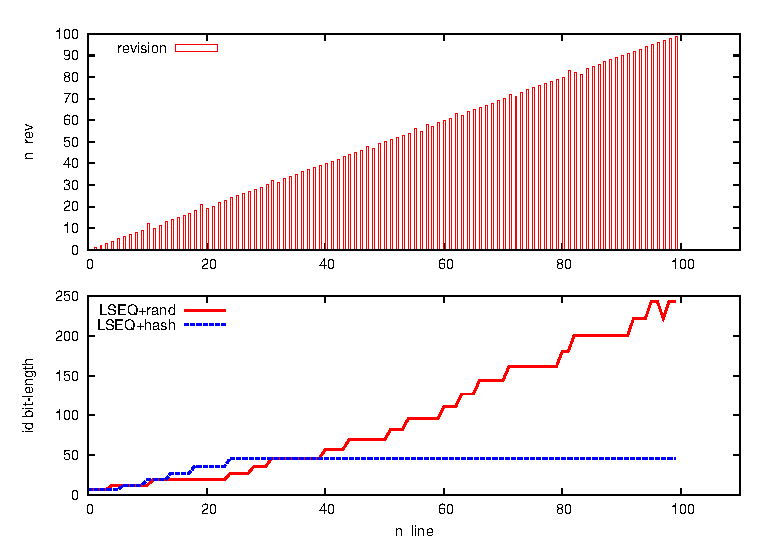
\includegraphics[width=0.49\textwidth]{img/tenusers.eps}
\caption{Experiments on a synthetic document of 100 lines edited at the end by
  10 collaborators (10 operations per user). The top figure shows the revision
  number of the operation. The bottom figure shows the bit-length of each
  identifier allocated to each line. On average, the bit-length of LSEQ and
  \NAME{} identifiers are 94.7 and 39.1 bit/id respectively.}
\label{im:tenusers}
\end{figure}


\subsection{Latency experiment}
\begin{asparadesc}
\item[Objective:] show that increasing the latency (the time between the
  generation and the delivery of an operation) does not imply a growth in the
  size of identifiers. On the contrary, when the latency increases, the average
  size of allocated identifiers decreases. This behaviour is expected on both
  LSEQ and \NAME{} that use a random strategy choice and a hash strategy choice
  respectively.
\item[Description:] we simulate a set of 10 collaborators producing a document
  of 100 lines. Each one of these collaborators performs 10 insert operations
  at the end of the document. The users generate operations following the
  Poisson distribution of parameter $\lambda=100$. i.e. users more likely
  generate an operation after 100 rounds (arbitrary unit) from their previous
  operation. Measurements are done at a latency of 5, 10, 20, 40, 80, 160, 320,
  640 rounds. They concern the average bit-length of identifiers in the
  document.  We evaluate two setups: the random strategy choice \textbf{rand}
  and the hash strategy choice \textbf{hash} using the allocation strategies
  $boundary+$ and $boundary-$ with $boundary=10$ and departure
  $base=2^{4+depth}$.
\item[Results:] Figure~\ref{im:stats} shows the results of the latency
  experiments. As expected, the two setups allocate identifiers with an average
  bit-length that quickly decreases when the latency increases. Therefore, the
  latency does not badly affect LSEQ and \NAME{} allocation strategies. Also,
  it confirms observations made in previous experiment: \textbf{hash} performs
  better than \textbf{rand} especially on low latency.
\item[Reasons:] increasing the latency delays the arrival of operations to the
  remote collaborators. Thus, each collaborator works locally until it delivers
  the operation generated by other users. Considering the extreme case with the
  maximum latency, each collaborator generates its 10 insertions, and then
  merges the others' 90 operations. Consequently, the 100 operations share the
  same space, i.e., the digit part of identifiers can be the same for multiple
  elements, and the total order is maintained by the source and clock.
\end{asparadesc}


\begin{figure}
\begin{center}
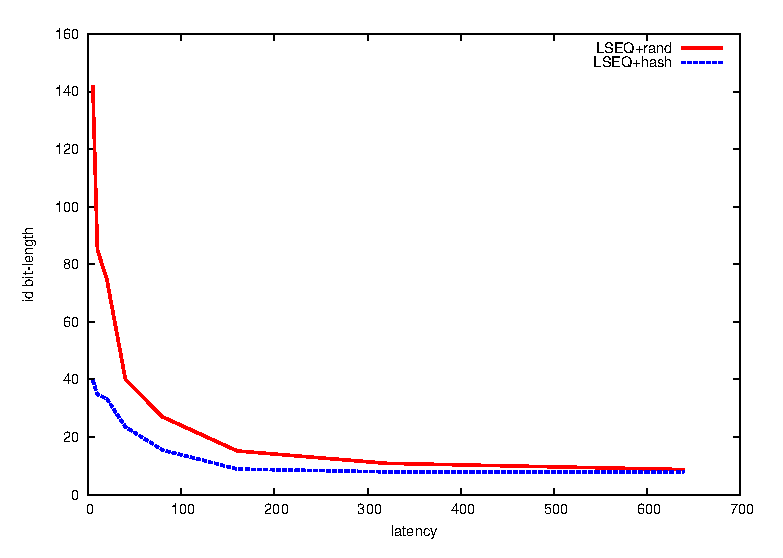
\includegraphics[width=0.49\textwidth]{img/stats.eps}
\caption{Experiments of latency effects over the average bit-length of
  identifiers. A group of 10 collaborators generates a synthetic document of
  100 lines (10 operations each). Two configurations of LSEQ: the original
  random strategy choice and the hash strategy choice (\NAME{}).}
\label{im:stats}
\end{center}
\end{figure}

\subsection{Synthesis}
The experiments evaluated the effect of concurrency on the average bit-length
of identifiers by varying the number of collaborators and the latency. They
showed that an implicit and \emph{a priori} agreement on allocation strategy
choices is required to maintain the sub-linear upper-bound on space
complexity. Employing the same hash function to chose the allocation strategy
permits to reach this agreement. Consequently, the improvement of LSEQ called
\NAME{} can be safely used in distributed collaborative editing. The latency
experiment shows that increasing the latency parameter only results in sharing
the identifier space, and consequently lowers the size of identifiers. As a
corollary, considering an immediate delivery of operations constitutes a
sufficient upper-bound on the behaviour of the overall system under higher
latency.

%%% Local Variables: 
%%% mode: latex
%%% TeX-master: "../dchanges"
%%% End: 

  
\section{Related Work}
\label{sec:relatedwork}
Current distributed collaborative editors uses optimistic
replication~\cite{saito2002replication,saito2005optimistic} to provide
availability of data at a consistency cost. Optimistic replication designs
operation in two phases. First a replica prepares the result of an operation
and then broadcasts it to other collaborators. Second, remote replicas
integrat the newly received data.

Operational Transform approach (OT) and Conflict-free Replicated Data Type
approach (CRDT) belong to the optimistic class of replication. While CRDTs
share the computational cost of operations between the local and remote parts
of the replication protocol, the OT approaches prefer to offer free local
generation and pay an additional cost on integration of remote operations.
Since the number of remote operations exponentially grows when the number of
collaborators increases, the CRDTs scale better than OT approaches.


We distinguish two classes of CRDTs for sequences. The tombstone based CRDT
approaches use death certificate on removed elements. Henceforth, these
elements are hidden to the users, but still remain in the underlying model and
undermine the performance. For instance, the number of tombstones in popular or
controversial pages in Wikipedia pages would be very high due to vandalism and
recoveries. The representatives of this class of CRDTs are
WOOT~\cite{oster2006data}, WOOTO~\cite{weiss2007wooki},
WOOTH~\cite{ahmed2011evaluating}, CT~\cite{grishchenko2010deep},
Treedoc~\cite{preguica2009commutative}, PPS~\cite{wu2010partial},
RGA~\cite{roh2011replicated} and \cite{Yu2012stringwise}.

To get rid of these marked elements, the tombstone based CRDTs require
additional protocols related to garbage collecting
mechanisms. In~\cite{letia2009crdts,roh2011replicated} they propose approaches
to safely purge the tombstones. However, it requires a global knowledge over
collaborators.  In~\cite{roh2011replicated}, they describe an approach that
obtains the global knowledge by maintaining a vector clock with one entry per
participant although it is too costly in large distributed network where
collaborators can enter and leave the system. In~\cite{letia2009crdts}, they
describe the \emph{core nebula} approach that permits to reach the consensus
over participants. However, this approach constrains the network topology to
make the consensus reachable and uses a costly catch up protocol.

The alternative to tombstones is the variable-size identifiers CRDT
approach. These CRDTs directly encode the total order of elements into their
unique identifiers. Thus, they do not require tombstones however the
identifiers can grow. In Logoot~\cite{weiss2009logoot} and
Treedoc~\cite{preguica2009commutative}, identifiers have a linear space
complexity compared to the number of insert operations. Furthermore, their size
heavily depends on the position of insertions. For example, performing
insertions repetitively at the beginning of a document leads to identifiers
with a size equals to the number of insert operations. Consequently, such
approaches require an additional re-balance protocol, like tombstone CRDTs.
However their underlying allocation strategies can be replaced by
LSEQ~\cite{nedelec2013lseq} that provides a sub-linear upper-bound on the space
complexity regardless of the editing behaviour.

The LSEQ approach uses two antagonist allocation strategies. However, while
paper~\cite{ahmed2011evaluating} argues about the importance of concurrency in
CRDTs experiments, the original paper of LSEQ does not consider this aspect. In
this paper, we showed on synthetic documents that its original configuration
does not scale in the number of users. The added value of synthetic documents
over real collaborative documents is the total flexibility on their parameters,
especially on the editing behaviour. Indeed, the number of available real
collaborative documents (including concurrency) is very limited. Moreover, such
experiments are costly to set up, and often biased by the nature of the task to
perform.


In this paper, we propose to replace the random strategy choice component of
LSEQ by a hash strategy choice component to reach an implicit consensus on
which strategy to employ. This configuration called \NAME{} does not require
additional computation and extends the sub-linear complexities of LSEQ from a
single user to multiple collaborators regardless of the latency. Thus, \NAME{}
constitutes a safe allocation strategy for sequences CRDTs, even in cases
including concurrency.


%%% Local Variables: 
%%% mode: latex
%%% TeX-master: "../dchanges"
%%% End: 

  
\section{Conclusion}

In this paper, we presented an improvement of the allocation strategy LSEQ
called \NAME{}. Contrarily to the original approach, our configuration supports
multiple users regardless of the latency. Indeed, replacing the random strategy
choice by the hash strategy choice allows to reach a global sub-linear
upper-bound on space complexity. As a consequence, distributed collaborative
editors can safely use \NAME{} and show better scalability criteria than
current trending editors such as Google Docs, Etherpad, etc.

The hash strategy choice is a common function over participants that maps a
depth in the underlying tree to an allocation strategy identifier. This
surjective function initialized with a shared seed allows to reach an agreement
on strategies with no additional synchronization. Consequently, there is no
loss in the identifier space due to antagonist allocation strategies.

This paper highlights the importance of multiple users analysis in CRDTs for
sequences, particularly in the case of multiple underlying allocation
strategies. We also showed that latency does not badly affect the size of
identifiers in variable-size identifiers CRDTs. However, we performed
experiments with synthetic documents in order to show the general behaviour of
the allocation without considering semantically consistent documents.

Future works include the formal proof of the sub-linear upper-bound on space
complexity of \NAME{}. A probability analysis of the worst-case scenario is
mandatory to show that it seldom happens. We plan to experiment \NAME{} on a
corpus of real documents including multiple collaborators and
concurrency. Finally, we aim to build a real distributed collaborative editor
based on a variable-size identifiers CRDT using \NAME{} as allocation strategy.

%%% Local Variables: 
%%% mode: latex
%%% TeX-master: "../dchanges"
%%% End: 


%% Bibliographie
%  \newpage
  \bibliographystyle{abbrv}
  \raggedright
  \bibliography{bibliographie}
%  \addcontentsline{toc}{chapter}{Bibliographie} 
%  \nocite{*}
  \clearpage
  
\end{document}
